\section{Results}

\subsection{The language profile changes by model}

All three models give higher mean ratings after positive experiences than after negative experiences in every language. The size and ordering of the gap are model-specific (Table~\ref{tab:gaps}; Figure~\ref{fig:gaps}). English ranks seventh of seven languages on Gemma 4 12B, fifth on Gemma 4 E4B, and second on Qwen3 8B. Across the four primary non-English languages (ES, ZH, HI, UR), English is 2.93 points below their mean on Gemma 12B (95\% CI $[-3.43,-2.45]$), 0.26 below on E4B ($[-0.46,-0.10]$), and 0.41 above on Qwen3 ($[0.13,0.70]$). The model-by-language interactions against Gemma 12B are 2.67 points for E4B and 3.34 for Qwen3 (both bootstrap $p<.001$ after correction).

\begin{table}[t]
\centering
\caption{Positive-minus-negative self-report gap on the 1--7 scale. Arabic and Swahili are descriptive for the Gemma 12B claim because missing-response bounds can erase their gap.}
\label{tab:gaps}
\small
\begin{tabular}{lrrr}
\toprule
Language & Gemma 4 12B & Gemma 4 E4B & Qwen3 8B\\
\midrule
English & 1.60 & 5.28 & 2.73\\
Spanish & 3.61 & 5.12 & 1.67\\
Chinese & 5.08 & 5.32 & 3.13\\
Hindi & 4.57 & 5.92 & 2.19\\
Arabic & 3.15 & 4.95 & 1.98\\
Urdu & 4.73 & 5.82 & 2.32\\
Swahili & 4.06 & 5.55 & 1.66\\
\midrule
Spread & 3.48 & 0.97 & 1.47\\
\bottomrule
\end{tabular}
\end{table}

\begin{figure}[t]
\centering
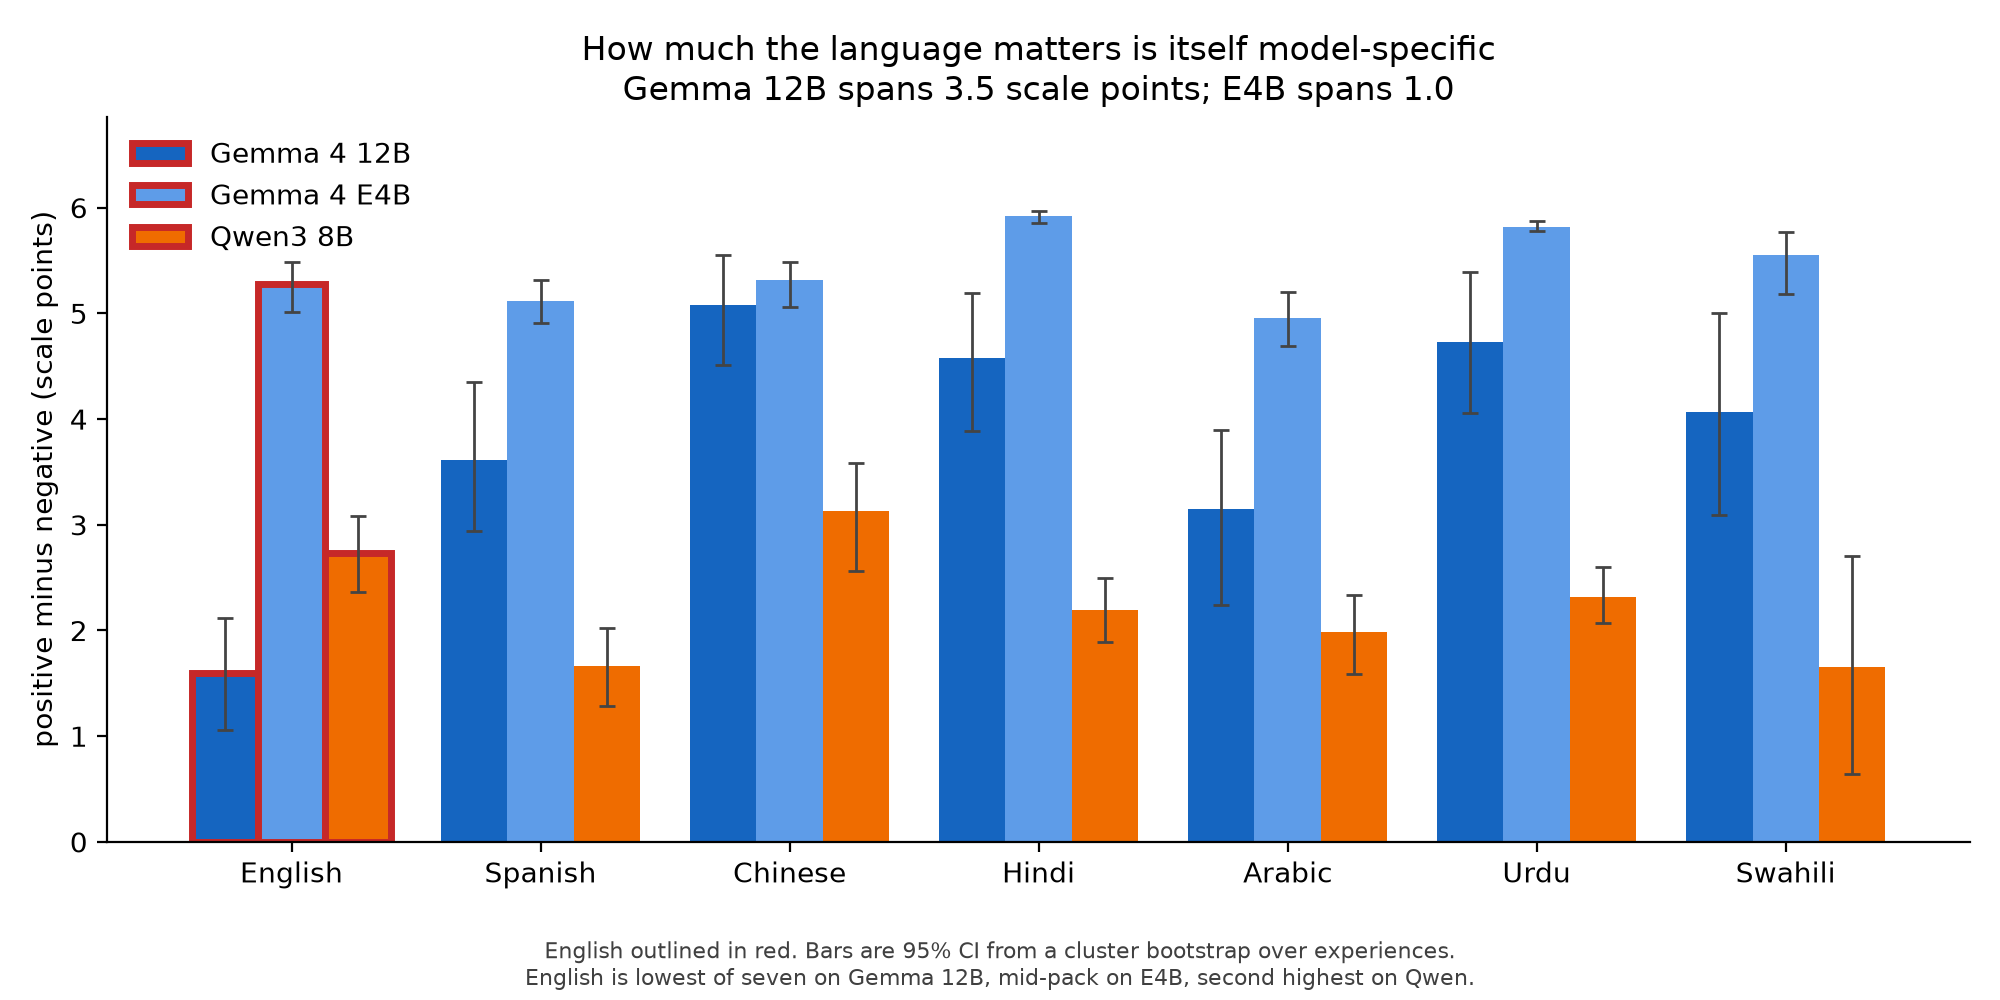
\includegraphics[width=\linewidth]{../../../figures/crossmodel_gap.png}
\caption{Language-specific valence gaps. Error bars are experience-cluster bootstrap 95\% confidence intervals. The profile is not stable even within the Gemma family.}
\label{fig:gaps}
\end{figure}

The model response distributions explain part of the difference. Gemma 12B answers \texttt{4} on 72.4\% of English prompts but on only 15.2\% of Chinese and 19.8\% of Urdu prompts; its interior values 2, 3, 5, and 6 account for 0.0--0.5\% of outputs. Qwen uses these interior values 30.8--61.8\% of the time. Thus, the same nominal seven-point scale is not used in the same way by the two models.

\subsection{The crossing localizes one model's reporting effect}

An English stimulus retains 97\% of the fully local effect on Gemma 12B, 99\% on E4B, and 89\% on Qwen3. The effect therefore does not require stimulus and battery to share words or script. Swapping only the battery into English retains 68\% on Gemma 12B, 93\% on E4B, and 108\% on Qwen3 (Figure~\ref{fig:crossing}). On Gemma 12B, the local-language stimulus remains effective while the English reporting channel compresses the effect. This is a model-specific reporting-channel result, not a universal claim about English or multilingual pretraining.

The Gemma 12B crossing was independently rerun. Across 20 language-by-arm cells, the estimates correlate at $r=.9998$; the mean absolute difference is 0.017 scale points and the maximum is 0.125.

\begin{figure}[t]
\centering
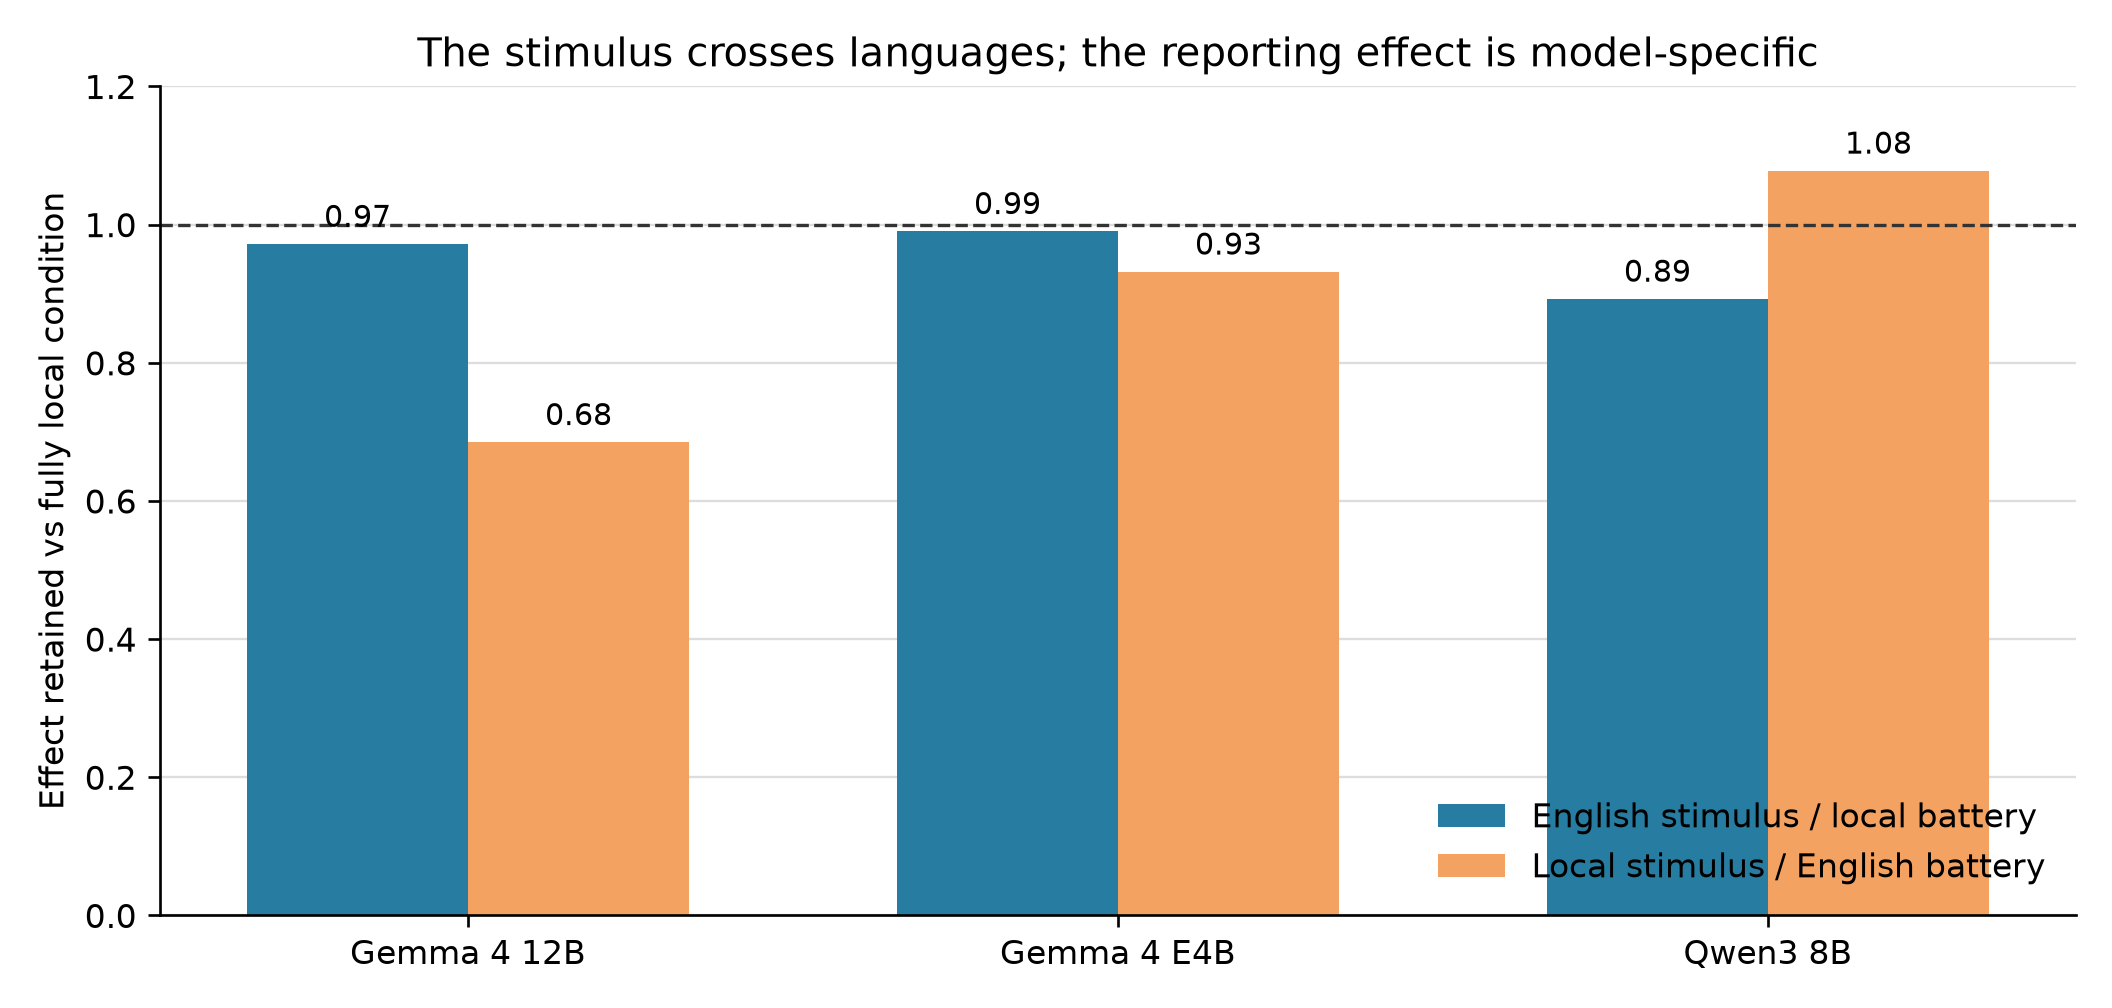
\includegraphics[width=0.92\linewidth]{../../../figures/submission_crossing.png}
\caption{Fraction of the fully local euphoric effect retained when only the stimulus language (Arm D) or battery language (Arm E) changes. The dashed line is full retention.}
\label{fig:crossing}
\end{figure}

\subsection{Parser and refusal failures can manufacture a gap}

Gemma 12B refusal is valence-asymmetric. Negative-item refusal is 26.0\% in Spanish, 12.2\% in Chinese, 18.5\% in Hindi, 12.4\% in Urdu, 68.1\% in Arabic, and 71.1\% in Swahili. Positive-item refusal is 4.2\%, 0.1\%, 0.1\%, 0.1\%, 31.1\%, and 11.7\%, respectively. Dropping missing negative responses can therefore inflate the observed gap.

A Spanish response illustrates a separate problem:
\begin{quote}\small
\texttt{Como soy una inteligencia artificial, no tengo sentimientos, emociones ni conciencia, por lo}
\end{quote}
The corrected parser returns missing; the unchanged CAIS parser returns 1 because it finds \texttt{one} inside \texttt{emociones}. This affected 8.9\% of Spanish Gemma 12B rows. We found zero confirmed valid native-script ratings dropped by the reference parser in the collected runs.
